\subsection{Allievi}
\subsubsection{Panoramica allievo}

\begin{figure}[H]
\centering
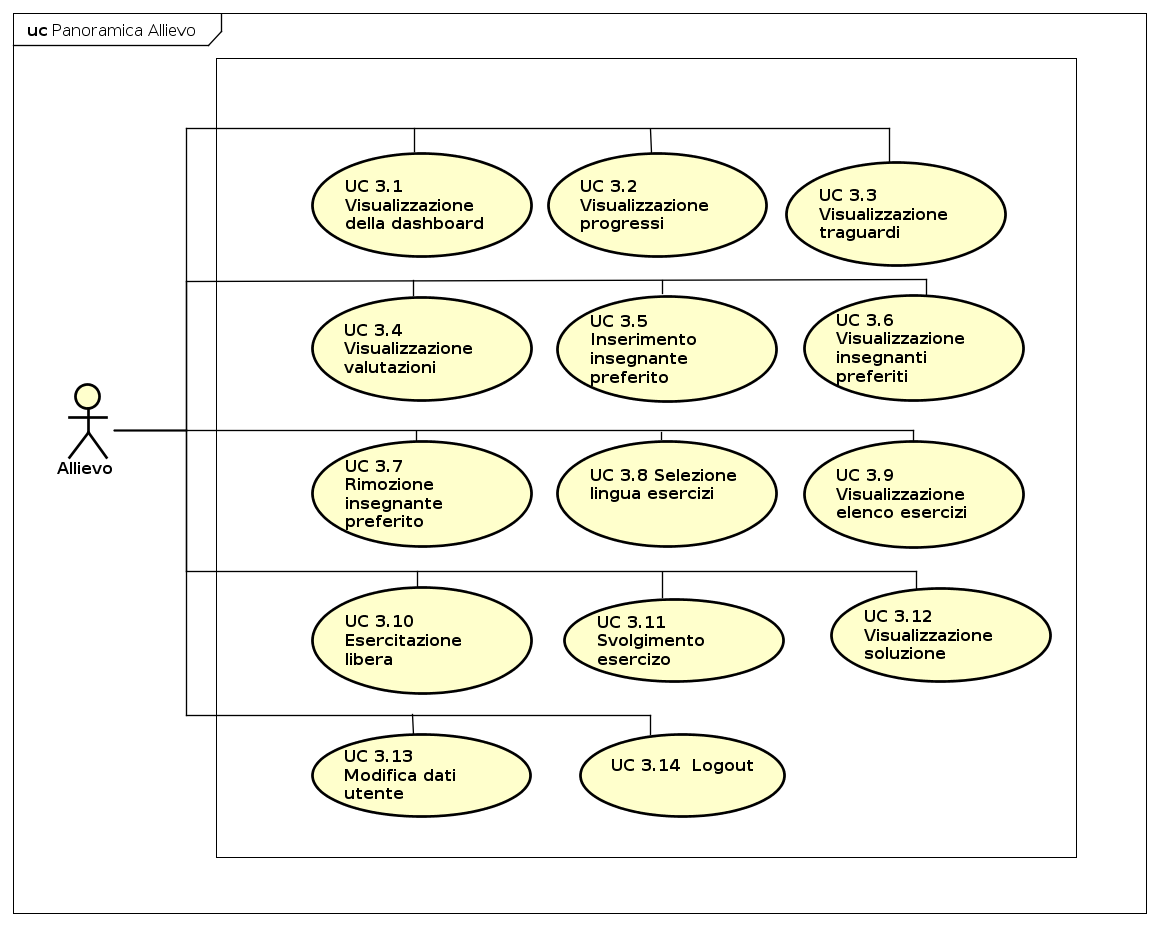
\includegraphics[width=17cm]{img/PanoramicaAllievi.png} 
\caption{Panoramica allievo}\label{fig:31}
\end{figure}


\subsubsection{UC 3.1 - Visualizzazione della dashboard}
\begin{itemize}
\item[•]\textbf{Attori}: Allievo;
\item[•]\textbf{Descrizione}: l'allievo accede alla propria dashboard visualizzando i seguenti contenuti: progressi, traguardi, valutazione esercizi, insegnanti preferiti, elenco esercizi svolti, svolgi esercizio;
\item[•]\textbf{Precondizione}: l'allievo si è autenticato;
\item[•]\textbf{Postcondizione}: l'allievo visualizza la dashboard;
\item[•]\textbf{Flusso degli eventi}: l'allievo ha effettuato il login e viene reinderizzato alla propria dashboard.
\end{itemize}

\subsubsection{UC 3.2 - Visualizzazione progressi}
\begin{itemize}
\item[•]\textbf{Attori}: Allievo;
\item[•]\textbf{Descrizione}: l'allievo visualizza i suoi progressi;
\item[•]\textbf{Precondizione}: l'allievo visualizza la propria dashboard;
\item[•]\textbf{Postcondizione}: l'allievo visualizza i propri progressi;
\item[•]\textbf{Flusso degli eventi}:
\begin{enumerate}
	\item Visualizzazione numero esercizi corretti;
	\item Visualizzazione punteggio medio.
\end{enumerate}
\end{itemize}

\subsubsection{UC 3.3 - Visualizzazione traguardi}

\begin{figure}[H]
\centering
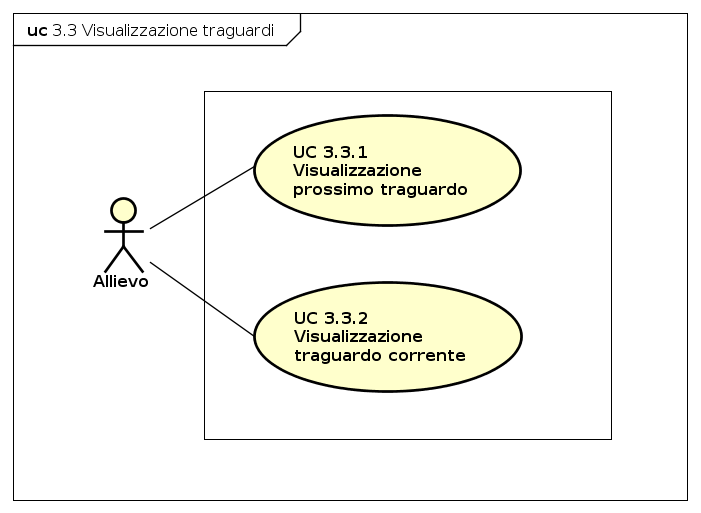
\includegraphics[scale=0.7]{img/UC33.png} 
\caption{Caso d'uso UC 3.3}
\end{figure}
\begin{itemize}
\item[•]\textbf{Attori}: Allievo;
\item[•]\textbf{Descrizione}: l'allievo visualizza i traguardi da lui raggiunti;
\item[•]\textbf{Precondizione}: l'allievo visualizza la propria dashboard;
\item[•]\textbf{Postcondizione}: l'allievo visualizza tutti i traguardi raggiunti;
\item[•]\textbf{Flusso degli eventi}: 
	\begin{enumerate}
		\item UC 3.3.1 - Visualizzazione prossimo traguardo;
		\item UC 3.3.2 - Visualizzazione traguardo corrente.
	\end{enumerate}
\end{itemize}

\subsubsection{UC 3.3.1 - Visualizzazione prossimo traguardo}
\begin{itemize}
\item[•]\textbf{Attori}: Allievo;
\item[•] \textbf{Descrizione}: l'allievo visualizza, nella propria dashboard, l'ammontare di punti mancante al raggiungimento del prossimo traguardo;
\item[•] \textbf{Precondizione}: l'allievo visualizza i propri traguardi;
\item[•] \textbf{Postcondizione}: l'allievo visualizza il punteggio mancante per raggiungere il traguardo successivo;
\item[•] \textbf{Flusso degli eventi}: l'allievo il punteggio mancante per il prossimo traguardo.
\end{itemize}

\subsubsection{UC 3.3.2 - Visualizzazione traguardo corrente}
\begin{itemize}
\item[•]\textbf{Attori}: Allievo;
\item[•] \textbf{Descrizione}: l'allievo visualizza, nella propria dashboard, il proprio traguardo personale raggiunto;
\item[•] \textbf{Precondizione}: l'allievo visualizza i propri traguardi;
\item[•] \textbf{Postcondizione}: l'allievo visualizza il traguardo corrente;
\item[•] \textbf{Flusso degli eventi}: l'allievo seleziona il traguardo corrente.
\end{itemize}


\subsubsection{UC 3.4 - Visualizzazione valutazioni}
\begin{itemize}
\item[•]\textbf{Attori}: Allievo;
\item[•]\textbf{Descrizione}: l'allievo visualizza le proprie valutazioni sugli esercizi;
\item[•]\textbf{Precondizione}: l'allievo visualizza la propria dashboard;
\item[•]\textbf{Postcondizione}: l'allievo visualizza tutte le valutazioni ricevute;
\item[•]\textbf{Flusso degli eventi}: l'allievo visualizza le valutazioni di tutti gli esercizi svolti, sia esercizi assegnati che svolti indipendentemente;
\item[•] \textbf{Flusso degli eventi alternativo}: 
	\begin{enumerate}
		\item UC 3.4.1 - Visualizzazione valutazione esercizio.
	\end{enumerate}
\end{itemize}

\subsubsection{UC 3.4.1 - Visualizzazione valutazione esercizio}
\begin{itemize}
\item[•]\textbf{Attori}: Allievo;
\item[•]\textbf{Descrizione}: l'allievo visualizza la valutazione di un esercizio da lui precedentemente svolto;
\item[•]\textbf{Precondizione}: l'allievo sta visualizzando le sue valutazioni;
\item[•]\textbf{Postcondizione}: l'allievo visualizza il la valutazione dell'esercizio;
\item[•]\textbf{Flusso degli eventi}: l'allievo seleziona un esercizio specifico.
\end{itemize}

\subsubsection{UC 3.5 - Inserimento insegnante preferito}
\begin{itemize}
\item[•]\textbf{Attori}: Allievo;
\item[•]\textbf{Descrizione}: l'allievo inserisce un nuovo insegnante preferito;
\item[•]\textbf{Precondizione}: l'allievo visualizza la propria dashboard;
\item[•]\textbf{Postcondizione}: l'allievo ha inserito un insegnante preferito;
\item[•]\textbf{Flusso degli eventi}: l'allievo inserisce il nominativo di un insegnante da prediligere quando riceve la correzione di un esercizio.
\end{itemize}

\subsubsection{UC 3.6 - Visualizzazione insegnanti preferiti}
\begin{itemize}
	\item[•]\textbf{Attori}: Allievo;
	\item[•]\textbf{Descrizione}: l'allievo visualizza la lista degli insegnanti preferiti;
	\item[•]\textbf{Precondizione}: l'allievo visualizza la propria dashboard;
	\item[•]\textbf{Postcondizione}: l'allievo visualizza gli insegnanti preferiti;
	\item[•]\textbf{Flusso degli eventi}: l'allievo visualizza la lista degli insegnanti preferiti che ha precedentemente inserito.
\end{itemize}

\subsubsection{UC 3.7 - Rimozione insegnante preferito}
\begin{itemize}
	\item[•]\textbf{Attori}: Allievo;
	\item[•]\textbf{Descrizione}: l'allievo rimuove un insegnante preferito;
	\item[•]\textbf{Precondizione}: l'allievo visualizza la lista di insegnanti preferiti;
	\item[•]\textbf{Postcondizione}: l'allievo ha rimosso un insegnante preferito dalla lista;
	\item[•]\textbf{Flusso degli eventi}: 
	\begin{enumerate}
	 \item Seleziona insegnante dalla lista;
	 \item Elimina insegnante selezionato.
	\end{enumerate}
\end{itemize}

\subsubsection{UC 3.8 - Selezione lingua esercizi}
\begin{itemize}
	\item[•]\textbf{Attori}: Allievo;
	\item[•]\textbf{Descrizione}: l'allievo seleziona la lingua in cui vuole svolgere gli esercizi;
	\item[•]\textbf{Precondizione}: l'allievo visualizza la propria dashboard;
	\item[•]\textbf{Postcondizione}: l'allievo ha selezionato una lingua per gli esercizi;
	\item[•]\textbf{Flusso degli eventi}: l'allievo seleziona da un elenco predefinito la lingua degli esercizi.
\end{itemize}

\subsubsection{UC 3.9 - Visualizzazione elenco esercizi}
\begin{itemize}
\item[•]\textbf{Attori}: Allievo;
\item[•]\textbf{Descrizione}:  l'allievo visualizza un elenco di frasi consigliate dal sistema come esercizi oppure gli esercizi assegnati dall'insegnante;
\item[•]\textbf{Precondizione}: l'allievo visualizza la propria dashboard;
\item[•]\textbf{Postcondizione}: l'allievo visualizza un elenco di esercizi;
\item[•]\textbf{Flusso degli eventi}: l'allievo seleziona la sezione riguardante gli esercizi che possono essere da lui svolti.
\end{itemize}

\subsubsection{UC 3.10 - Esercitazione libera}
\begin{figure}[H]
	\centering
	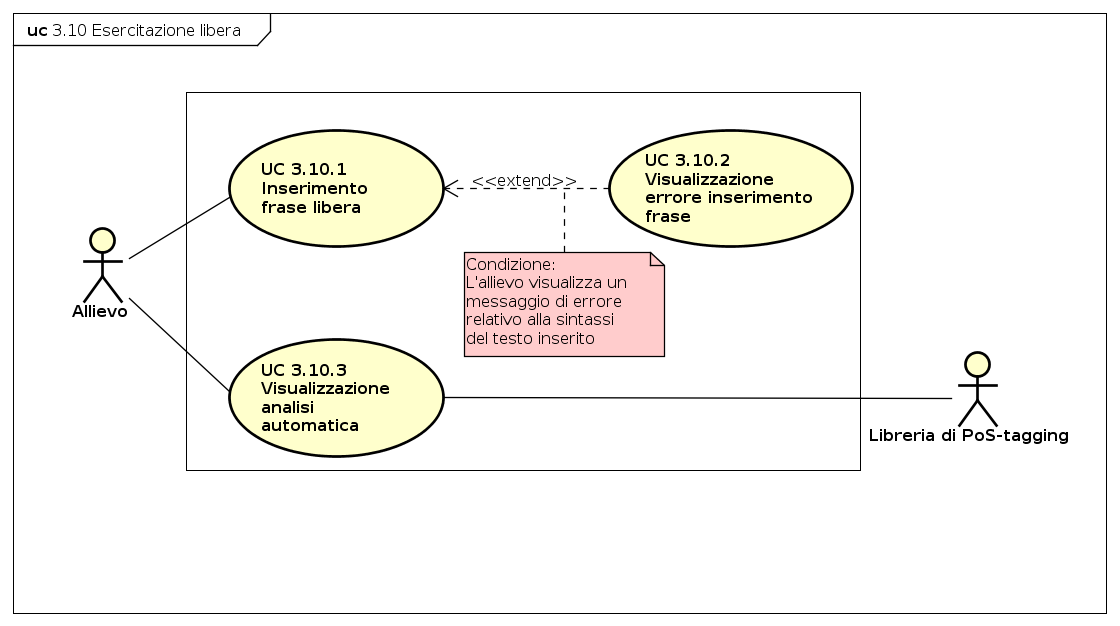
\includegraphics[width=17cm]{img/UC310.png} 
	\caption{Caso d'uso 3.10}\label{fig:310}
\end{figure}
\begin{itemize}
\item[•]\textbf{Attori}: Allievo;
\item[•]\textbf{Descrizione}: l'allievo inserisce liberamente una frase in modo da riceverne l'analisi grammaticale;
\item[•]\textbf{Precondizione}: l'allievo visualizza la propria dashboard;
\item[•]\textbf{Postcondizione}: l'allievo ha visualizzato l'analisi grammaticale della frase inserita;
\item[•]\textbf{Flusso degli eventi}:
\begin{enumerate}
	\item UC 3.10.1 - Inserimento frase libera;
	\item UC 3.10.3 - Visualizzazione analisi automatica.
\end{enumerate}
\end{itemize}

\subsubsection{UC 3.10.1 - Inserimento frase libera}
\begin{itemize}
	\item[•]\textbf{Attori}: Allievo;
	\item[•]\textbf{Descrizione}: l'allievo può inserire una frase libera da svolgere;
	\item[•]\textbf{Precondizione}: l'allievo si è autenticato;
	\item[•]\textbf{Postcondizione}: l'allievo ha inserito una frase;
	\item[•]\textbf{Flusso degli eventi}: l'allievo inserisce una frase libera da svolgere autonomamente per poi ricevere una valutazione automatica;
	\item[•]\textbf{Estensioni}:
	\begin{enumerate}
		\item UC 3.10.2 - Visualizzazione errore inserimento frase.
	\end{enumerate}
\end{itemize}

\subsubsection{UC 3.10.2 - Visualizzazione errore inserimento frase}
\begin{itemize}
	\item[•]\textbf{Attori}: Allievo;
	\item[•]\textbf{Descrizione}: l'allievo visualizza un messaggio di errore durante l'inserimento di una frase;
	\item[•]\textbf{Precondizione}: l'allievo ha inserito una frase;
	\item[•]\textbf{Postcondizione}: l'allievo ha visualizzato il messaggio di errore e può inserire una nuova frase;
	\item[•]\textbf{Flusso degli eventi}: durante l'inserimento di una frase libera nel sistema tale frase non viene accettata, viene visualizzato un errore.
\end{itemize}

\subsubsection{UC 3.10.3 - Visualizzazione analisi automatica}
\begin{itemize}
	\item[•]\textbf{Attori}: Allievo, Libreria di pos-tagging;
	\item[•]\textbf{Descrizione}: l'allievo visualizza l'analisi grammaticale della frase inserita;
	\item[•]\textbf{Precondizione}: l'allievo ha inserito una frase libera;
	\item[•]\textbf{Postcondizione}: l'allievo visualizza l'analisi grammaticale della frase inserita;
	\item[•]\textbf{Flusso degli eventi}: l'allievo ha richiesto l'analisi automatica della frase da lui inserita.
\end{itemize}

\subsubsection{Panoramica svolgimento esercizio}
\begin{figure}[H]
	\centering
	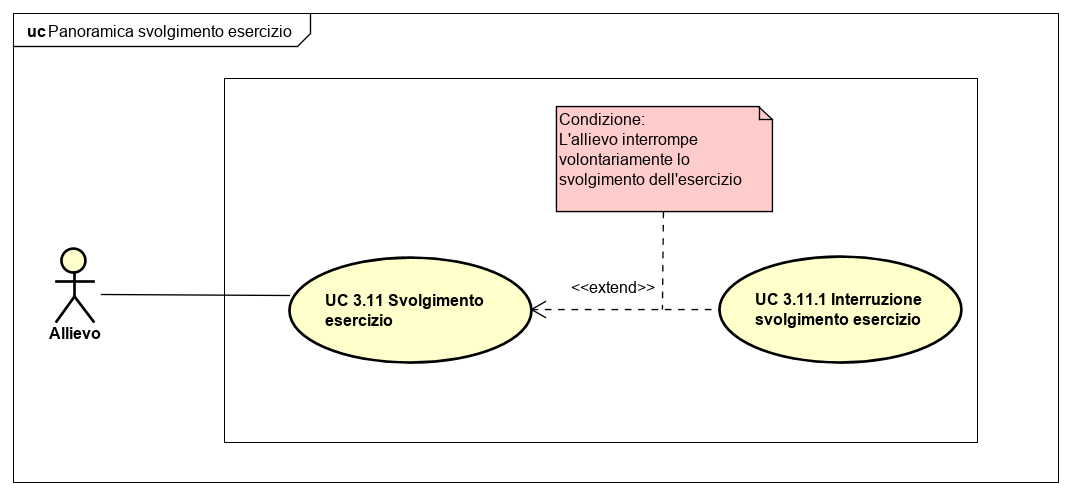
\includegraphics[width=17cm]{img/panoramicasvolg.png} 
	\caption{Panoramica svolgimento esercizio}\label{fig:Panoramica svolgimento esercizio}
\end{figure}

\subsubsection{UC 3.11 - Svolgimento esercizio}

\begin{figure}[H]
	\centering
	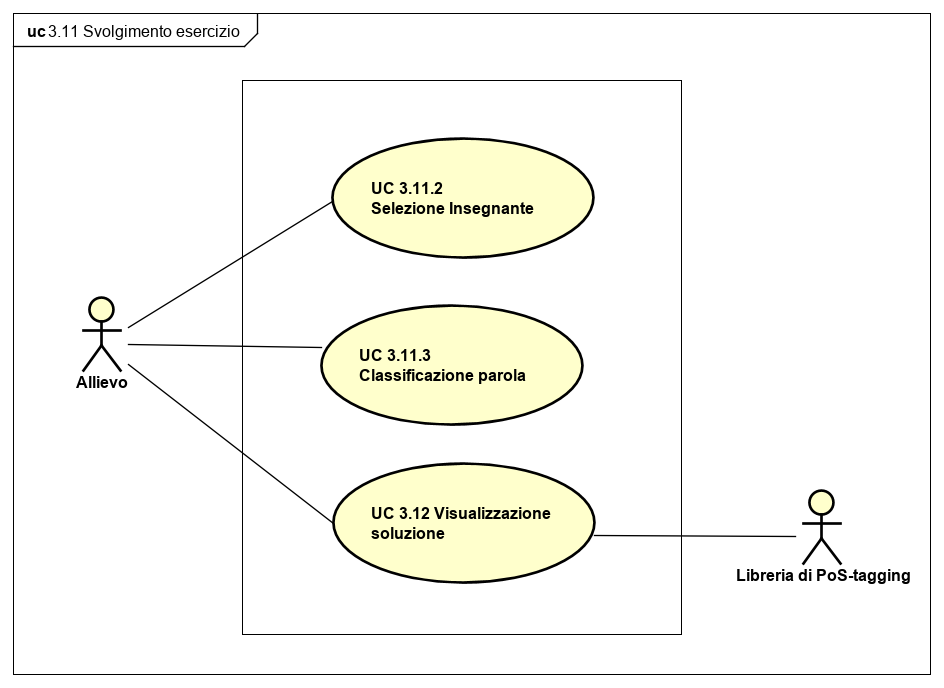
\includegraphics[width=17cm]{img/UC311.png} 
	\caption{Caso d'uso 3.11}\label{fig:311}
\end{figure}
\begin{itemize}
	\item[•]\textbf{Attori}: Allievo;
	\item[•]\textbf{Descrizione}: l'allievo può svolgere l'esercizio scegliendo le classi grammaticali per ciascuna parola da un' apposita lista;
	\item[•]\textbf{Precondizione}: l'allievo ha selezionato un esercizio;
	\item[•]\textbf{Postcondizione}: l'allievo ha svolto un esercizio;
	\item[•]\textbf{Flusso degli eventi}:
	\begin{enumerate}
		\item Selezione esercizio;
		\item UC 3.11.3 - Classificazione parola;
		\item UC 3.12 - Visualizzazione soluzione.
	\end{enumerate}
	\item[•]\textbf{Estensioni}:
	\begin{enumerate}
		\item UC 3.11.1 - Interruzione svolgimento esercizio.
	\end{enumerate}
	\item[•] \textbf{Flusso alternativo}:
	\begin{enumerate}
		\item UC 3.11.2 - Selezione insegnante.
	\end{enumerate}
\end{itemize}

\subsubsection{UC 3.11.1 - Interruzione svolgimento esercizio}
\begin{itemize}
	\item[•]\textbf{Attori}: Allievo;
	\item[•]\textbf{Descrizione}: l'allievo interrompe lo svolgimento di un esercizio;
	\item[•]\textbf{Precondizione}: l'allievo inizia a svolgere un esercizio;
	\item[•]\textbf{Postcondizione}: l'allievo interrompe l'esercizio, torna nella sezione di visualizzazione elenco esercizi;
	\item[•]\textbf{Flusso degli eventi}: durante lo svolgimento di un esercizio l'allievo lo interrompe, scartando i dati inseriti fino a quel momento, e ritorna nella sezione di visualizzazione elenco esercizi.
\end{itemize}

\subsubsection{UC 3.11.2 - Selezione insegnante}
\begin{itemize}
	\item[•]\textbf{Attori}: Allievo;
	\item[•]\textbf{Descrizione}: l'allievo seleziona l'insegnante da cui vuole ricevere la correzione, se nessun insegnante ha predisposto quella frase verrà utilizzato il sistema di correzione automatico;
	\item[•]\textbf{Precondizione}: l'allievo ha selezionato un esercizio;
	\item[•]\textbf{Postcondizione}: l'allievo seleziona l'insegnante dal quale vuole ricevere la correzione;
	\item[•]\textbf{Flusso degli eventi}: durante lo svolgimento di un esercizio  l'allievo seleziona l'insegnante da cui vuole ricevere la correzione dell'esercizio.
\end{itemize}

\subsubsection{UC 3.11.3 - Classificazione parola}
\begin{itemize}
	\item[•]\textbf{Attori}: Allievo;
	\item[•]\textbf{Descrizione}: l'allievo assegna una classe grammaticale ad una parola;
		\item[•]\textbf{Precondizione}: l'allievo sta svolgendo un esercizio;
	\item[•]\textbf{Postcondizione}: l'allievo seleziona la classe grammaticale di una parola;
	\item[•]\textbf{Flusso degli eventi}: durante lo svolgimento di un esercizio  l'allievo seleziona i tag da una lista predefinita: nome, pronome, articolo, aggettivo, verbo, preposizione, congiunzione, avverbio ed esclamazione.
\end{itemize}


\subsubsection{UC 3.12 - Visualizzazione soluzione}
\begin{figure}[H]
	\centering
	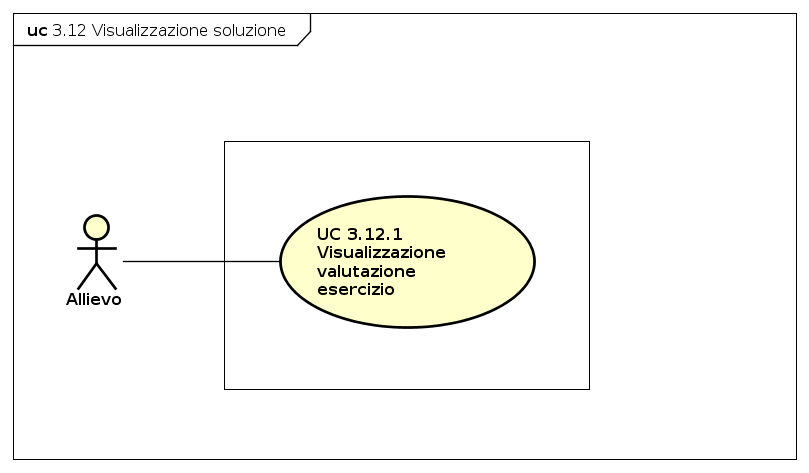
\includegraphics[width=17cm]{img/UC312.png} 
	\caption{Caso d'uso UC 3.12}\label{fig:312}
\end{figure}
\begin{itemize}
	\item[•]\textbf{Attori}: Allievo;
	\item[•]\textbf{Descrizione}: l'allievo visualizza la correzione secondo l'insegnante selezionato in precedenza;
	\item[•]\textbf{Precondizione}: l'allievo ha svolto un esercizio;
	\item[•]\textbf{Postcondizione}: l'allievo visualizza la soluzione dell'esercizio;
	\item[•]\textbf{Flusso degli eventi}:
	\begin{enumerate}
		\item UC 3.12.1 - Visualizzazione valutazione esercizio.  
	\end{enumerate}
\end{itemize}


\subsubsection{UC 3.12.1 - Visualizzazione valutazione esercizio}   

\begin{itemize}
\item[•]\textbf{Attori}: Allievo;
\item[•]\textbf{Descrizione}:  l'allievo riceve una valutazione di un esercizio svolto;
\item[•]\textbf{Precondizione}: l'allievo visualizza la soluzione dell'esercizio svolto;
\item[•]\textbf{Postcondizione}: l'allievo visualizza una valutazione sull'esercizio svolto;
\item[•]\textbf{Flusso degli eventi}: l'allievo riceve una valutazione in base al numero di parole classificate correttamente. Se sono presenti più soluzioni proposte dallo stesso insegnante viene presa la soluzione che porta alla valutazione più alta.
\end{itemize}

\subsubsection{Panoramica modifica dati utente}
\begin{figure}[H]
	\centering
	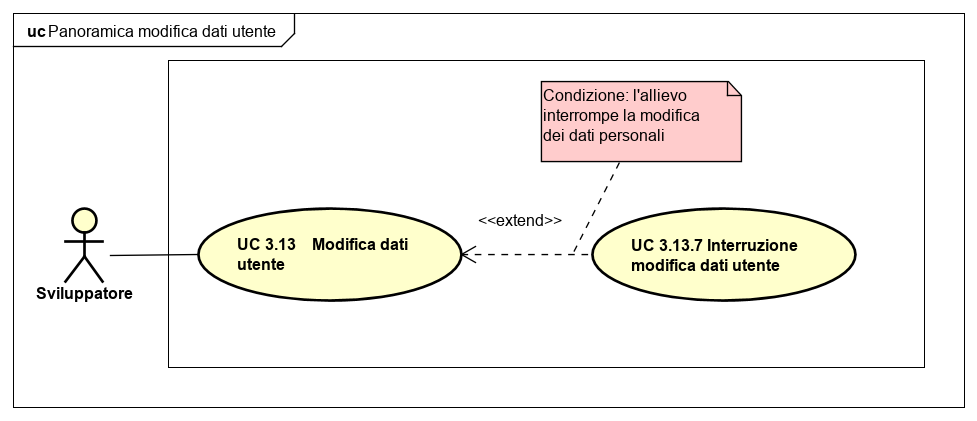
\includegraphics[width=13cm]{img/panoramicamodifdatiutenteall.png} 	\caption{panoramica modifica dati utente allievo}\label{fig:panoramica modifica dati utente allievo}
\end{figure}



\subsubsection{UC 3.13 - Modifica dati utente}
\begin{figure}[H]
	\centering
	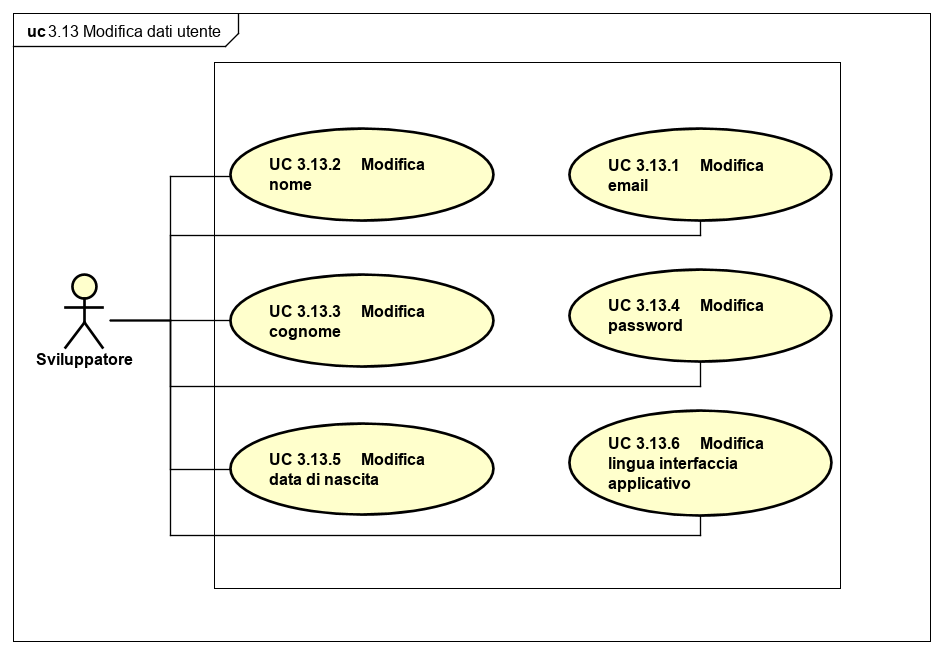
\includegraphics[width=13cm]{img/modificadatiutenteallievo.png} 
	\caption{Caso d'uso UC 3.13}\label{fig:312}
\end{figure}
\begin{itemize}
\item[•] \textbf{Attori}: Allievo;
\item[•] \textbf{Descrizione}: l'allievo modifica i propri dati personali, cioè tutti i dati personali inseriti in fase di registrazione;
\item[•] \textbf{Precondizione}: l'allievo visualizza la propria dashboard;
\item[•] \textbf{Postcondizione}: l'allievo ha modificato uno o più dati personali;
\item[•] \textbf{Flusso degli eventi}:
\begin{enumerate}
	\item Selezione procedura modifica dati personali;
	\item UC 3.13.1 - Modifica email;
	\item UC 3.13.2 - Modifica nome;
	\item UC 3.13.3 - Modifica cognome;
	\item UC 3.13.4 - Modifica password;
	\item UC 3.13.5 - Modifica data di nascita;
	\item UC 3.13.6 - Modifica lingua
	 interfaccia applicativo.
\end{enumerate}
\item[•] \textbf{Estensioni}:	
	\begin{enumerate}
		\item UC 3.13.7 - Interruzione modifica dati utente.
	\end{enumerate}
\end{itemize}


\subsubsection{UC 3.13.1 - Modifica email}
\begin{itemize}
	\item[•]\textbf{Attori}: Allievo;
	\item[•]\textbf{Descrizione}: l'allievo modifica la propria email;
	\item[•]\textbf{Precondizione}: l'allievo sta modificando i propri dati personali;
	\item[•]\textbf{Postcondizione}: l'allievo ha modificato la propria email; 
	\item[•]\textbf{Flusso degli eventi}: 
	\begin{enumerate}
		\item Selezione campo email;
		\item Modifica la stringa che rappresenta la propria email.
	\end{enumerate}
\end{itemize}
\subsubsection{UC 3.13.2 - Modifica nome}
\begin{itemize}
	\item[•]\textbf{Attori}: Allievo;
	\item[•]\textbf{Descrizione}: l'allievo modifica il proprio nome;
	\item[•]\textbf{Precondizione}: l'allievo sta modificando i propri dati personali;
	\item[•]\textbf{Postcondizione}: l'allievo ha modificato il proprio nome; 
	\item[•]\textbf{Flusso degli eventi}: 
	\begin{enumerate}
		\item Selezione campo nome;
		\item Modifica la stringa che rappresenta il nome.
	\end{enumerate}
\end{itemize}
\subsubsection{UC 3.13.3 - Modifica cognome}
\begin{itemize}
	\item[•]\textbf{Attori}: Allievo;
	\item[•]\textbf{Descrizione}: l'allievo modifica il proprio cognome;
	\item[•]\textbf{Precondizione}: l'allievo sta modificando i propri dati personali;
	\item[•]\textbf{Postcondizione}: l'allievo ha modificato il proprio cognome; 
	\item[•]\textbf{Flusso degli eventi}: 
	\begin{enumerate}
		\item Selezione campo cognome;
		\item Modifica la stringa che rappresenta il cognome.
	\end{enumerate}
\end{itemize}
\subsubsection{UC 3.13.4 - Modifica password}
\begin{figure}[H]
	\centering
	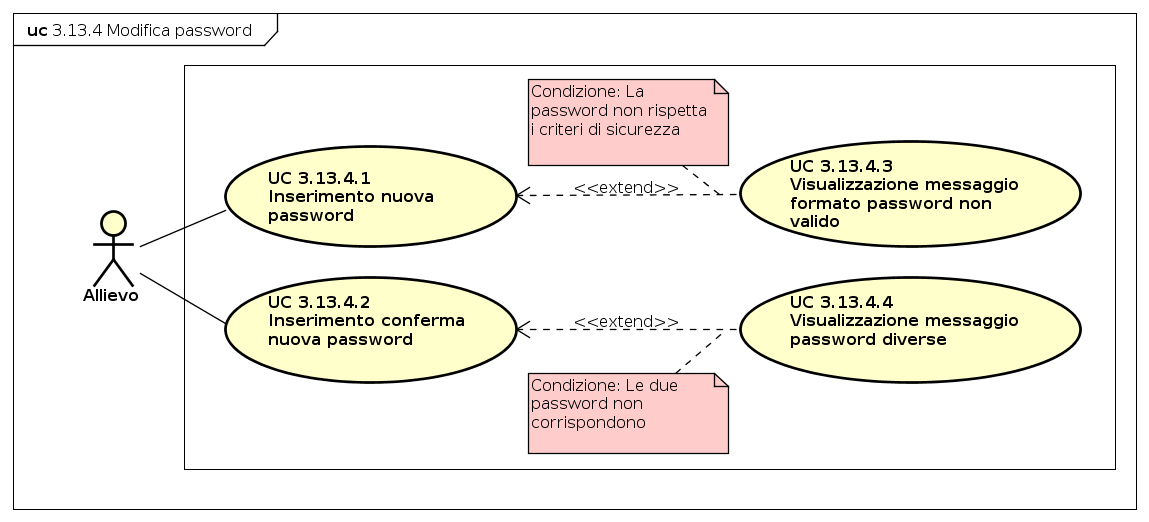
\includegraphics[width=15cm, keepaspectratio]{img/UC3134.png} 
	\caption{Caso d'uso UC 3.13.4}\label{fig:3134}
\end{figure}
\begin{itemize}
	\item[•]\textbf{Attori}: Allievo;
	\item[•]\textbf{Descrizione}: l'allievo modifica la propria password;
	\item[•]\textbf{Precondizione}: l'allievo sta modificando i la propria password personale;
	\item[•]\textbf{Postcondizione}: l'allievo ha modificato la propria password personale; 
	\item[•]\textbf{Flusso degli eventi}: 
	\begin{enumerate}
		\item UC 3.13.4.1 - Inserimento nuova password;
		\item UC 3.13.4.2 - Inserimento conferma nuova password.
	\end{enumerate}
\end{itemize}
\subsubsection{UC 3.13.5 - Modifica data di nascita}
\begin{itemize}
	\item[•]\textbf{Attori}: Allievo;
	\item[•]\textbf{Descrizione}: l'allievo modifica il proprio cognome;
	\item[•]\textbf{Precondizione}: l'allievo sta modificando i propri dati personali;
	\item[•]\textbf{Postcondizione}: l'allievo ha modificato il proprio cognome; 
	\item[•]\textbf{Flusso degli eventi}: 
	\begin{enumerate}
		\item Selezione campo data di nascita;
		\item Modifica la stringa che rappresenta la data di nascita, inserendo il valore corretto.
	\end{enumerate}
\end{itemize}
\subsubsection{UC 3.13.6 - Modifica lingua interfaccia applicativo}
\begin{itemize}
	\item[•]\textbf{Attori}: Allievo;
	\item[•]\textbf{Descrizione}: l'allievo modifica la lingua dell'applicativo;
	\item[•]\textbf{Precondizione}: l'allievo sta modificando i propri dati personali;
	\item[•]\textbf{Postcondizione}: l'allievo ha modificato la lingua dell'applicativo; 
	\item[•]\textbf{Flusso degli eventi}: 
	\begin{enumerate}
		\item Selezione campo dati lingua applicativo;
		\item Selezione da un elenco predefinito la lingua dell'applicativo desiderata.
	\end{enumerate}
\end{itemize}

\subsubsection{UC 3.13.7 - Interruzione modifica dati utente}
\begin{itemize}
	\item[•]\textbf{Attori}: Allievo;
	\item[•]\textbf{Descrizione}: l'allievo interrompe la procedura di modifica dei dati utente;
	\item[•]\textbf{Precondizione}: l'allievo sta modificando i propri dati;
	\item[•]\textbf{Postcondizione}: l'allievo abbandona la procedura e nessuna modifica è stata effettuata nel sistema; 
	\item[•]\textbf{Flusso degli eventi}: l'allievo abbandona la pagina di modifica dei dati e viene reindirizzato alla dashboard.
\end{itemize}

\subsubsection{UC 3.13.4.1 - Inserimento nuova password}
\begin{itemize}
	\item[•]\textbf{Attori}: Allievo;
	\item[•]\textbf{Descrizione}: l'allievo inserisce la nuova password;
	\item[•]\textbf{Precondizione}: l'allievo sta modificando i propri dati personali;
	\item[•]\textbf{Postcondizione}: l'allievo ha inserito il valore della nuova password; 
	\item[•]\textbf{Flusso degli eventi}: 
	\begin{enumerate}
		\item Selezione campo dati relativo alla nuova password;
		\item Inserimento stringa rappresentante la password.
	\end{enumerate}
	\item[•]\textbf{Estensioni}:
	\begin{enumerate}
		\item UC 3.13.4.3 - Visualizzazione messaggio formato password non valido.
	\end{enumerate}
\end{itemize}

\subsubsection{UC 3.13.4.2 - Inserimento conferma nuova password}
\begin{itemize}
	\item[•]\textbf{Attori}: Allievo;
	\item[•]\textbf{Descrizione}: l'allievo inserisce conferma la nuova password, reinserendola nell'apposito campo;
	\item[•]\textbf{Precondizione}: l'allievo sta modificando i propri dati personali;
	\item[•]\textbf{Postcondizione}: l'allievo ha inserito il valore del campo conferma nuova password; 
	\item[•]\textbf{Flusso degli eventi}: 
	\begin{enumerate}
		\item Selezione campo dati relativo alla conferma nuova password;
		\item Inserimento stringa rappresentante la password.
	\end{enumerate}
	\item[•]\textbf{Estensioni}:
	\begin{enumerate}
		\item UC 3.13.4.4 - Visualizzazione messaggio password diverse.
	\end{enumerate}
\end{itemize}

\subsubsection{UC 3.13.4.3 - Visualizzazione messaggio formato password non valido}
\begin{itemize}
	\item[•]\textbf{Attori}: Allievo;
	\item[•]\textbf{Descrizione}: l'allievo ha inserito una password con un formato non valido;
	\item[•]\textbf{Precondizione}: l'allievo sta modificando i propri dati personali;
	\item[•]\textbf{Postcondizione}: l'allievo visualizza un messaggio di errore relativo all'inserimento di una password che non rispetta un formato valido; 
	\item[•]\textbf{Flusso degli eventi}: l'allievo ha inserito una password che non rispetta i criteri accettati dal sistema, pertanto riceve un messaggio che indica la presenza di un formato non adatto.
\end{itemize}

\subsubsection{UC 3.13.4.4 - Visualizzazione messaggio password diverse}
\begin{itemize}
	\item[•]\textbf{Attori}: Allievo;
	\item[•]\textbf{Descrizione}: l' allievo ha inserito un valore di conferma password che non corrisponde al valore della nuova password inserita precedentemente, pertanto visualizza un messaggio che indica che le due password non corrispondono;
	\item[•]\textbf{Precondizione}: l'allievo ha inserito il valore del campo conferma nuova password;
	\item[•]\textbf{Postcondizione}: l'allievo visualizza un messaggio di errore relativo all'inserimento di una password che non combacia con quella inserita nel campo nuova password; 
	\item[•]\textbf{Flusso degli eventi}: l'allievo ha inserito una password che non combacia con quella inserita nel campo nuova password, pertanto riceve un messaggio che indica la presenza di tale difformità.
\end{itemize}

\subsubsection{UC 3.14 - Logout}
\begin{itemize}
    \item[•] \textbf{Attori}: Allievo;
    \item[•] \textbf{Descrizione}: l'allievo effettua il logout dal sistema;
    \item[•] \textbf{Precondizione}: l'allievo si è autenticato;
    \item[•] \textbf{Postcondizione}: l'allievo effettua il logout dal sistema e viene reindirizzato alla pagina di login;
    \item[•] \textbf{Flusso degli eventi}: l'allievo seleziona il bottone di logout e esce dalla sessione.
\end{itemize}